\documentclass[a4paper,10pt]{article}

\usepackage{raskolnikov}
\title{Pigeoncide project}
\subtitle{Analysis of results}
%\date{Curso 07/08}
%\location{Universidad de Granada}
\author{Juan~Pedro~Bolívar~Puente\\Alberto~Villegas~Erce\\Marc~Modrow\\Sari~Sariola}

\begin{document}

\raskolnikovmaketitle
\tableofcontents

% \begin{abstract}
% \end{abstract}

\section{Introduction}

This document explains the arquitecture and features of the project
for the Introduction to Game Development course which took place in
the first semester in the Turun Yliopisto.

The game description was given in the proposal that we sent to the
evaluators in the firs week of the course, so we will move directly to
describing the given solution.

\section{How to read the source code}

The game source code is in the \texttt{src} folder of the distribution
package. Only a one-liner main file is included in that folder, the
rest of the code is included in subdirectories. To ease evaluating the
source code --and advancing an overview of the architecture-- we
describe what is in each of these folders, which are in a way layers
of the architecture. Trying to follow the layers from bottom up:

\begin{description}
\item[base] This module includes basic facilities that are common to
  any possible software application, such as generic implementations
  of design patterns, command line argument parsing, configuration
  storage and loading, etc...

\item[core] This module includes core facilities that are common to
  any possible game application. This includes the process managers,
  state managers, basic Panda3D management, timers, etc.

\item[phys] A thin and incomplete wrapper on top of ODE.

\item[ent] This include the entity system, providing a bunch of game
  independent entities. We discuss entities further later.

\item[game] The Pigeoncide specific game implementation.

\item[menu] The Pigeoncide menu system.

\item[app] The Pigeoncide concrete app facilities.

\item[test] Unit tests for many of the modules.

\end{description}

\section{Game architecture}

The whole project was writen in Python ($2.2 < version < 3$) using the
Panda3D\cite{gosling04panda3d} game framework. Panda3D is a highly featured system,
including a whole bunch of interesting features such as a physics
engine --actually two of them, a simple one and an ODE\cite{odephysics}
wrapper-- to a scene graph 3D engine and sound systems.

However, we soon found that its design didn't really fit our
expectatives, at least when it comes to architectural aspects. They
can not be blamed for that though, as their objective is not to
provide a well engineered architecture, but a very featured scripting
facility that resembles more a \emph{domain specific language} built
on top of Python than just a game development framework\footnote{This
  explains why they \emph{abuse} Python features and insist on
  injecting their global variables --which should be punished anyway--
into the \texttt{\_\_builtins\_\_} module.}. Their purpose
is to have small game scripts coded fast, leaving features such as
scalability and manageability of the code apart.

\subsection{Resource management and hierarchy}

One of the biggest problems that we saw in the Panda3D system is the
insistence on using global state. Even worse than that, the global
state was used most of the time implicitly, by using either the global
variables installed as Python built-ins, or using many of the
facilities of \texttt{DirectObject} that installed event listeners
and other entities into global systems via calls to apparently local
methods.

Resource management has been and is still one of the biggest problems
in computer programming and that kind of practices does not help at
all. Sadly, the belief that \emph{garbage collection} has vanished all
resource management problems has not done anything else than making
the problem worse, as leaking memory is not the worst problem of
resource management, and it is easy to see badly programmed Java
applications leaving a system blocked because it was leaking SQL
connections\footnote{No offence, but Java seems to be a honey pot for
  resource leaks, probably because of its attraction to frustrated
  C/C++ programmers looking for the relief of garbage collection.}.

Maybe biased by our deep experience with languages supporting the
\emph{Resource Adquisition Is Initialization} idiom\footnote{We will
  not say names, because the lecturers made their language preferences
  clear during the course ;)} is we believe that hierarchy is a good thing. This
hierarchy, can be made explicit by the means of \emph{lexical scope}
--such as in the RAII case-- or class design such as the
\emph{composite}\cite{gamma95design} pattern. Panda3D properly implements this
in the scene graph. 

We take this one step further and make other basic game engine
sub-systems hierarchical, providing easier means to control
resources, these are: the \texttt{task} system, the \texttt{event}
system, and our \texttt{state} system. Let's discuss them further now.

\subsection{Abstracting the game loop}

Most computer games share a common basic structure: a game loop that
iterates gathering the use input, updating the state in response to
the input and the previous state, and updating the output to reflect
these changes. This game loop iterates around many times per second
--usually 60 or so.

For this purpose we implemented a \texttt{task} module that abstracts
the game loop. This is a well know game pattern and described in books
such as \cite{mcshaffry03game}, so we will not step deeply in its
description. The important question here is \emph{why did we
  re-implement a feature that was already in Panda3d?}. We answer the
question here:

\begin{enumerate}
\item Because of resource management. Many entities in the game may
  generate many tasks that have to be executed. However, the task
  system provided with Panda3D is flat, and therefore one could not do
  such a simple thing as ``pause all the tasks belonging to this
  object''. The solution for us was to have a hierarchical task
  manager, where one object could hold its own local task
  manager. This way, for example, using \texttt{pause ()} on the local
  task manager will pause all its child tasks.

  We had an interesting discussion about this in the Panda3D with one
  of its main developers\cite{pandataskforum}. There, when asked about the
  convenience of re-implementing the task manager the Panda3D
  developer argued that we would loose nice features that they
  implement such as the graphical task browser that he found very
  useful in the debugging process. We finally decided that a
  hierarchical task manager would not leak tasks and therefore would
  not need such a tool, and this has proven to be true. When asked
  about how to group related tasks together, he suggested giving them
  a name such as \texttt{``parent-taskname''} and removing them by
  using blobs like \texttt{``parent-*''}. The fact that Panda3D
  implements such things as finding tasks using blobs clearly reflects
  a feature overkill that could be made not needed by using a proper
  design\footnote{Re-reading this, it can seem a bit harsh... I am not
    arguing that Panda3D developers are unable to come up with proper
    design, and I really believe that they have done a great
    job.. Once again, I feel that those kind of features are very
    useful for unexperienced developers willing to make
    quick-and-dirty games, which is the main target audience of
    Panda3D.}.

\item Many features of their task system seemed too heavy for us. Every
  task is identified and managed through a string. Also, they where
  ordered using priority queues, what makes adding and deleting tasks
  logarithmic. We wanted to be able to abuse the task system adding
  and deleting them all the time --preferably in constant time-- and
  we did not find the need for string identification for them, etc.
\end{enumerate}

So we came up with a nice and small task system that is the basis
for all the game, and can be further studied in the
\texttt{core.task} module in the source package of our game. In our
design, a \texttt{TaskGroup} is the task manager, but it is also a
\texttt{Task}, so they can be hierarchically composed easily. Like
in Panda3D, simple functions can be used as tasks too. We also
provide a bunch of utility tasks in that module that, combined with
lambda's and such make it really easy to write complex animations
and interactions in a one-liner --such as \texttt{task.sequence},
\texttt{task.parallel}, \texttt{task.wait}, \texttt{task.fade},
... These utility tasks cover most of what Panda3D call
\emph{intervals} and are very easily implemented thanks to our
design. Once again, one could argue that Panda3D intervals are more
featured, but I argue that most of those features are not needed ;)

Still, we believe that our system still have space for
improvements. The main interesting features that we can think of are
the support of multi-threading, and optional support for explicit task
ordering as done by Panda3D by assigning priorities. Also, it would be
nice for some kind of turn-based games that run on battery based
devices to have non-busy waits.

\subsection{The Hollywood principle: signals and events}
\label{sec:hollywood}
The so-called \emph{Hollywood principle} states that ``you should not
call us, leave your script and we will call you.'' That is the essence
of modern object oriented programming and the Model-View-Controller
architectural pattern that this game implements. In this, the view
leave a \emph{reference} in the model, so they get notified when the
controller alters it. To achieve this, most of the time the
\emph{observer}\cite{gamma95design} and \emph{multicast}\cite{vlissides98pattern} design
patterns come handy.

Slot-signal libraries usually provide a generic implementation of the
pattern\footnote{Pattern orthodoxes find this statement a bit awkward,
as patterns are not reusable pieces of code but reusable pieces of
design. However, it is a fact that modern computer languages can
implement patterns with reusable code; a illuminating masterpiece in
this topic is Alexandrescu's \cite{alexandrescu01modern}. Also, some design
patterns are often implemented or superseded by language features,
specially in dynamic languages such as Python, but also we can see
this tendency in C\# delegates --observer pattern-- or Scala
object-class --singleton pattern.}.

\subsubsection{The \texttt{base.signal} module}

Because we knew before hand that we where going to use
\emph{observers} all along the project, the first thing that we
started to write just after the course began was the slot-signal
mechanism --along with the rest of the \texttt{base} module.

A \emph{signal} is an object that represents an event that can
ocurr. This is opposed to the event mechanism proposed in the course
and used by Panda3D, where events are string identifiers and all go
through the event manager. A \emph{slot} is an object that represents
a listening end on the signal. When the signal is invoked using either
the \texttt{notify ()} method or the convenient overloaded
\texttt{\_\_call\_\_} operator, the signal calls all the listening
slots, passing additional parameters if required. Slots are usually
arbitrary function objects.

The main problem with the signal mechanism is that they add complexity
for the resource management issue that we have discussed all along the
way, because it favours setting up complex object meshes that can be
hard to track. For this reason, we have implemented a bunch of
different facilities that ease this task, such as the
\texttt{weak\_slot} and \texttt{slot} decorators, and the
\texttt{Tracker} and \texttt{Trackable} classes implemented in
\texttt{base.connection}. Also a \texttt{base.observer} modules
provides easy means to generate whole signal based interfaces for
emitters and listeners, which helps in the task of wiring signal
connections where we are interested in a whole interface. The
implementation was very educative as it heavily uses
metaprogramming and advanced python features such as data descriptors,
decorators, and MRO based collaborative methods.

\subsubsection{Back to the Panda3D event system}

As we said, Panda3D uses a different approach to this, with an event
manager that dispatches all the signals, that are identified by
strings. One can listen on a concrete signal telling it to the event
manager. All the basic input handling is done in this way by Panda3D.

The main problem, once again, is that this event manager, called a
\texttt{messenger} in Panda3D, is global. We wanted some
form of scoping and hierarchy. We wrote a similar facility to Panda's
messenger, the \texttt{EventManager} in \texttt{base.event}, that,
while missing some unneeded features, was able to forward
all messages to other event managers. This way we got the needed
hierarchy: one can have its own event manager locally that can be used to receive all its parent signals, while still being
able to, for example, mute all its local subscribers. Also, this
system mapped the event system to the signal mechanism, providing
further convenience.

The only problem here was that Panda3D does not have the possibility
to have a ``catch-all'' method for its events. This was surprising
because that is one of the main advantages to have a event manager
instead of independent signal objects. To be able to forward Panda3D's
events to our event hierarchical system we only could modify the
Panda3D implementation. Because we wanted the game to be compatible
with third party distributions of the library, this was a no-no. But
then Python dynamism comes with an ugly but convenient technique to
solve this  paradox: \emph{monkey patching}. This is, modifying a class or
object's implementation at runtime. Our modifications are implemented in the
\texttt{core.messenger\_patch} module, which should be loaded
\emph{before} any other Panda3D module.

This has an important drawback: our game depends on Panda3D's
Messenger class implementation, and internal changes on it will break
it. It seems to work properly with version 1.6.X and 1.7 thought.

\subsection{Wiring everything up}

Specially in this MVC context, we end up with a mesh of objects that
communicate with each-other, in their role of either model state,
view, or controller. Someone else, a \emph{mediator}\cite{gamma95design}, have
to wire these things up.

On the other hand, we have been talking all the time that we have
carefully implemented hierarchical object structures in order to
achieve less coupling and local changes to certain \emph{scope}. The
question is, then how to define the scope of a game entity.

For these two purposes the \texttt{core.state} module comes into
hand. There we have a \emph{StateManager} and \emph{State} class. The
state manager provides a stack based state machine implementation. A
state can be something like a menu screen, a game, a loading screen,
etc. A game itself can be divided into different states, if needed. A
state is notified whenever it is no longer the top of the state stack,
and when it is again the top of the stack, for example. States,
combined with local managers, enable us to implement trivially 
otherwise not-so-easy features such pausing the game, having an
in-game menu, etc. Every state provides its own task manager and its
event manager.

The whole application is driven by states. The basic application
framework is abstracted in the \texttt{base.app} and refined to work
with states in \texttt{core.app}. From there onwards, one just
register states and moves around them by changing the current state,
entering a sub-state, leaving a state...

Also, the states are lightweight enough to be used to implement other
state machine based features such as AI. Still, there is a to-do note
in the state module talking about refactoring states to have an even
lighter version for such purposes in the future...


\subsection{Entities, a place for experimentation}
\label{sec:entities}
What is an ``entity''? An entity is an object inside the game
world. That is all what we can say about it. But, as for concrete
entities, we can say that:

\begin{enumerate}
\item They can have a lot of orthogonal features. For example, they
  can be a physical entity that reacts to its environment. It can be
  an entity represented visually by a 3D model, or an animated actor,
  or a 2D texture. Or it might be a physical entity, but that stands
  all the time, such as the player does. An infinite etcetera
  follows...

\item When writing a concrete entity, or an orthogonal feature for an
  entity, we want to concentrate on the logic that drives the entity
  or the feature that it adds, and not on boilerplate (a) resource
  management or (b) object wiring.
\end{enumerate}

During the course, the lecturers talked about event-driven
architecture, and at some point also about how things can actually get
messy --i.e. the example about the interactions between the physics
system and the scene graph. Also, while developing the \texttt{base}
module we had been learning a lot about advanced Python features, and
some background voice was asking for getting rid of all that
event-based thing to try to explore something... else. Then, we had
access to the BHive source code, the event based game engine developed
by the lecturers of this course, in order to find some inspiration.

The \texttt{world.WorldLinkers} module convinced us about trying a
different approach. The whole thing seemed too static for a dynamic
language, we thought.

The fact is that events, as used by BHive, provide a very nice way to
keep features orthogonal, as stated in our first requirement, but fail
in the second. What we propose in our experiment is something
different: using a language feature, \emph{multiple inheritance}, to
combine these orthogonal features of a single entity. MI! That is
evil! Well, not that much...

In (good) dynamic languages like Python, there is a nice feature
usually referred to as \emph{call-next-method}, after the name of the
function that implemented it in the Common Lisp's object system. In
Python, this is implemented using the \texttt{super} built-in that
returns the proxy of an object that calls the next method of a
class. This feature allows to call all the methods in a multiple
inheritance environment in a consistent order. This consistent order
is a linearization of the class hierarchy that satisfies the following
conditions:

\begin{enumerate}
\item If a class \texttt{Derived} inherits from a class \texttt{Base}
  then \texttt{Derived} comes first.
\item If a class \texttt{Derived} inherits form both class
  \texttt{BaseA} and \texttt{BaseB}, the \texttt{BaseA} also comes
  before \texttt{BaseB} --this is, there is left-to-right order in
  the same level of a hierarchy.
\item Every class appears only once in the linearization.
\end{enumerate}

Methods designed to work in this way --this is, they pass the control
to the \emph{super} class, where the \emph{super} is defined in the
previous terms\footnote{The C3 Method Resolution Order. Further
  literature can be read here \cite{pythonmro}\cite{barret96c3}.}--
are called collaborative, because they collaborate with \emph{unknown}
nodes in the class hierarchy. This feature is only possible in dynamic
languages, because the concrete type of \emph{super} inside a given
class can change when other classes derive from it\footnote{Still, we
  have an idea for some approximation for C++ in mind using heavy
  template metaprogramming...}. Much further can be said about how to
program using this technique, but this is not the purpose of this
text.

What is to be said, is that we use this to wire, implicitly, using
language features, the connections between these orthogonal
facilities of a game entity. When one of these features depends on some
other features, it derives from them. The C3 MRO ensures that these
dependencies will be correctly preserved even if the hierarchy gets
very complex, so no coupling is produced with other unrelated
features.

By using this, we solved problem 2.b. Also, to solve 2.a, the entity
system comes handy. The resources required for a given entity are
given by its entity manager. Every created entity is registered into
the entity manager that it receives in its constructor, and also keeps
a weak reference to it so it can use some shared resources at its
hierarchy level --for example, the task manager or event manager. Note that
entity managers can also be combined using this mix-ins
technique. There is also a \texttt{GameState} that specialises
\texttt{State} adding a entity manager that is set up with entity
manager able to hold visual an physical entities at a local scope,
something that is achieved, for example, by allocating its own node in
the scene graph. The entity manager is usually also in charge of
keeping track of all the entities for easy cleanup when we leave the
state, and it manage the entity resources; i.e. the
\texttt{PandaEntityManager} allocates a new node for the entity in the
scene graph on its creation, and removes it on its disposal. This can
be sometimes done with the collaboration of the entity itself.

Most of game independent entity facilities are developed inside the
\texttt{ent} submodules, while many specific ones are implemented in
the \texttt{game} module. We are very happy of how we achieved to
minimise boilerplate and maximise power. Still, some things can be
improved and the design is a bit experimental. The implementation is
plagued of to-do notes which are loud thoughts on how to improve the
design or the implementation. Much more can be said about this system,
for example, what \emph{decorators} and \emph{delegates} are in this
context, and how they are used to provide ``dynamic'' entities
--i.e. facilities that can be added and taken from an living
object. We make this more clear in later sections, but this text is getting too long, so we leave the code as a
testimony of it, and we are open to have discussions about this with
the evaluators of the course in person :)

\section{Implemented features}

We implement most of the features proposed in the course. We describe
in the following which of them and how.

\subsection{Hierarchical scene graph}

We use Panda3D hierarchical scene graph in all our graphical code. All
the entities into a game state are child of a sub-node of
\texttt{render} --this is, only the one node per state is in the
\texttt{render} root node to avoid its pollution. Each entity has its
own node, with the current state node as its parent. Some other
sub-nodes are used to tune the relative position of the parts of an
entity. We also use further features of the scene graph, such as
attaching the node of a weapon to the ``hand'' joint of the skeleton
of the animated boy, and properly using our entity combination system
to inject its coordinates to the physics system, etc.

\subsection{Physics}

We use the ODE wrapper distributed with Panda3D as physics engine. We
must say that this has been quite painful, for the following two
reasons:

\begin{enumerate}
\item ODE is very bad at solving the tunneling effect. This means that
  when the frame-rate drops, tunneling happens a lot, specially for
  fast entities. This was specially a problem for the pigeons, but we
  partially solved the problem by manually sweeping its collision
  volume\cite{ericson05collision}. The collision geometry of a pigeon was
  initially a sphere, but we changed it to be a cylinder that we use
  as a swept sphere whose length depends on the distance that the
  entity has moved in this frame.

  Still, the problem sometimes persists for other entities at low
  frame-rate and fast movement conditions. One solution is to try to
  keep the simulation running at a different frame-rate than the
  rendering, but this is less trivial as it might seem...

\item Either ODE or the Panda3D wrapper is plagued of bugs. When doing
  many apparently inoffensive things, but that ODE dislikes, it
  either segfaults or crashes the application with just a
  not-very-informative message. When debugging your application this
  makes it really a mess, because there is no way to backtrace the
  segmentation fault or ODE error to the Python code. Sometimes one
  can get a small backtrace of the C++ part of the wrapper executing Python
  inside \texttt{gdb}, but there is no way to know at which point of
  the Python script the problem occurred.
\end{enumerate}

Sadly, there is no Python wrapper for Bullet physics\cite{bulletphysics}
apart from the one embedded in the Blender Game Engine, so we do not
have a Free Software replacement for ODE in the near future.

\subsection{Event-based game logic}

We have not been very orthodox in implementing this, as explained in
section \ref{sec:entities}. However, our alternative architecture is
as capable or more than an event-based one. Also, the fact that we
did not use events to join together the different \emph{faces} of a world
object does not mean that we did not use events for other things like
one two many inter-entity communication.

As we described in \ref{sec:hollywood}, we have put a lot of effort in
implementing the generic low level components that are the basis of a
event based architecture. And we use events, all the time. They are
used to wire up most of the game logic. For example, when a physical
entity collides, it signals a \texttt{on\_collide} event, that is
listened by the \emph{killable} entity that it belongs to, that in
turn shows some particle effects and sounds, and then triggers the
\emph{on\_death} signal, that in turn is listened by a function that
finishes the game and enters the game over state for the player
entity. Or if the entity is a pigeon the \texttt{on\_death} signal is listened by a function that
increases the counter of dead pigeons and by another function that
checks whether there are more pigeons in the level to maybe enter the
game win state. This is just one simple example, but all our code is
plagued of this kind of event driven communication.

Also, while we did not go very further in this in our previous
description, while \emph{collaborative methods} are used to
communicate the different aspects of a single entity, events are used
to communicate among unrelated entities. Actually, an entity can be
\emph{observable} if it dispatches events on its spatial properties
updates. In this way, you can make a pigeon follow the boy or follow
some piece of food by changing no line of code apart from one that
changes which entity's events the pigeon listens to. The same happens
for the camera, and so on.

We even use events for the configuration system. Whenever a
configuration node is changed a signal is dispatched, allowing
unrelated listeners to be updated depending on the configuration state
--for example, when the music-volume option is changed, the menu can
listen to update the position of the scrollbar that changes the music
volume, and an object in charge of managing the Panda3D system changes
the volume parameter of the audio manager in charge of playing the
music.

So, while having an non canonical --but maybe better?-- implementation
of our events and entities systems, we definitely have a event based
architecture for gluing up almost all the application logic.

\subsection{MVC game architecture}

A consequence of the event based game logic is that we can easily come
up with a MVC game architecture. However, when we introduce the
\emph{mixin} based entities it might seem non-obvious how our
architecture is MVC. More exactly, how can be the views and
controllers of an entity decoupled from its state if they are combined
via inheritance?

There are three ways in which this is achieved, and the best one
depends on the concrete requirements:

\begin{enumerate}
\item First, there is the use of \emph{delegates} and \emph{decorators}
  system. If an entity mixin provides a delegate version of it, its
  controller can be dynamically changed using decorators. The
  decorator implementation is shared with the non-decorator version of
  the entity mixin, the only difference is that the decorator one
  controls its dependencies via a delegate --this is
  made in a transparent way, thanks to Python's magic. 

  The decorator can be seen as a controller that adds behaviour to a
  ``static'' model entity on runtime. For example, this code could be
  possible:

{\footnotesize
\begin{verbatim}
pigeon_model = mixin (PhysicalEntity) (entities = state.entities)
pigeon_controller = mixin (BoidEntityDecorator) (delegate = pigeon_model)
\end{verbatim}
}

One can think that this produces code duplication, because we need to
have two different versions of the \texttt{BoidEntity} and an
alternative controller version. However, the implementation can be
shared, and the following pattern arises when developing a controller
that can be used embedded with the model or as a separate object:

{\footnotesize
\begin{verbatim}
class BoidEntityBase (Entity):
   """
    Implementation of the flocking algorithm, asuming that all the
needed data is embedded into self.
   """
   ...

class BoidEntity (DynamicPhysicalEntity, BoidEntityBase): pass
class BoidEntityDecorator (DelegatePhysicalEntity, BoidEntityBase): pass
\end{verbatim}
}

The delegate is in charge of using \emph{properties} and functions to
forward all the interface that a \texttt{DynamicPhysicalEntity}
provides through another object. These delegates by now generate
a bit of boilerplate because the forwarding is encoded by hand, by we
are planning to adapt the functionality of \texttt{base.proxy} to
generate it automatically using Python's metaprogramming magic :)

\item Note that the previous code works only for wiring controllers
  with the model, because there is no way by which the decorator would
  be notified when the delegate changes, and, as such, we cannot
  connect a view to the model in this way.

  But, as the previous code shows, one can build the desired class on
  runtime mixing the needed entity components. For this, we provide
  the utility function \texttt{mixin} that creates a new class from a
  set of bases. For example, this code could be valid\footnote{We do
    not implement networked game, so some of the classes described are
    ficticious.}:

{\footnotesize
\begin{verbatim}
if game_is_local:
    pigeon = mixin (BoidEntity, DynamicPhysicalEntity, ActorEntity) (...)
elif game_is_client:
    pigeon = mixin (ActorEntity, RemotePhysicalEntity) (...)
elif game_is_server:
    pigeon = mixin (BoidEntity, DynamicPhysicalEntity, ServerPhysicalEntity) (...)
pigeon.set_position (100, 100, 100)
\end{verbatim}
}

In that way, the \emph{call-next-method} mechanism would make sure
that when a manipulation method is called on this model+view mixin
object it propagates correctly through all the hierarchy notifying the
views.

\item However, there is still a problem there. In the original MVC,
  one should be able to connect the model to many arbitrary instances of
  a view --in a mixin we can have one instance per view type only. Also, in the previous example one can not change the
  connections of the model with the views after the object is built,
  because they are embedded in the class hierarchy of the object.

  For this purpose, we can fall-back to the events mechanism,
  extending the entities interface with signals and events. This
  example code shows how this can be made, for example, connecting a
  follower camera to a pigeon.

{\footnotesize
\begin{verbatim}
class FollowCameraEntity (Entity, Trackable, SpatialEntityListener):
    ...

boy    = mixin (Boy,    ObservableSpatialEntity) (...)
pigeon = mixin (Pigeon, ObservableSpatialEntity) (...)
camera = FollowCameraEntity (...)
...
pigeon.connect (camera)
...
camera.disconnect_sources () # Method added by Trackable
boy.connect (camera)
...
# If it was not a trackable we have to remember who it was connected to.
boy.disconnect (camera) 
\end{verbatim}
}
\end{enumerate}

As we can see, we provide a nice way to separate algorithms from the
needs of the object topology. They should specify their requirements
inheriting from interfaces that are implemented in different ways, and
then later combined in runtime.

Note that because abstracting all needed Panda3D features in our
system is a lot of work, and because we sometimes took shortcuts in
our code for faster development --like skipping separating interface
and implementation-- our system might not always be as flexible as
previously shown if taken just outside the box. But the architecture not
only is MVC, but it can be more or less MVC depending on the concrete
needs of our system as previously shown, and only polishing a pair of
corners in the code is left to make the implementation 100\% loyal to
this explained methodology.

\subsection{Artificial Intelligence}

The pigeons movement is modelled using Craig Reynold's flocking
algorithm \cite{smed06algo}\cite{reynolds87flocks}. This allows to model the
complex behaviour of the flock of birds using autonomous agents with a
set of simple rules. We implemented it in a quite generic way --does not
depend on any kind of representation, being easy to combine with any
using our MVC architecture.

Also, that is not enough to model the complex behaviour of the
pigeons in our game. A state machine is used for this, with many states: fly,
walk, follow, fear, eat, hit, land, return, attack... Most of the
states just changes the parameters of the flocking algorithm, but some
of them do few extra things. The fact that they are implemented using
the state manager and our generic flocking algorithm makes the code
small and simple.

Sadly, our flocking implementation has an $O(n^2)$ time complexity,
being the biggest performance bottleneck of the application, and
making the application not very responsive when having a high number
of pigeons in the scene --more than 40 pigeons drops the framerate to
30 FPS in our computer and the tunneling problem of ODE becomes
significant. We are planning to improve this in the future by using
proper space partitioning to reduce the time complexity of the
algorithm, and even moving the core of the flocking
algorithm implementation to C or C++ code if needed.

\subsection{Lights and shaders}

We do not use many lights in the scene because we really do not needed
them much --or where very busy discovering the concepts behind our
experimental multi-paradigm architecture. Still, there is a light
on the top that provides some sunlight and an ambient light to avoid
excessively dark non-illuminated areas.

However, we still wanted to have nicer visuals, so we used \emph{glow
  mapping} to get nicely shaded laser fields and highlighted
sticks. We would use them in more places if it were not because of the
few problems that we had with the graphics --see the later section.

We implemented the glow mapping using a fragment shader
pipeline. First the whole scene is rendered to an off-screen buffer
using an alternative texture for each model (the glow map) that is combined with the normal one to
determine which regions should glow. Then that off-screen buffer is
blurred using two shaders, one that blurs the texture vertically and
another one that blurs it horizontally. Then, this buffer is merged on
top of the normally rendered scene, resulting in a very nice glow
effect.

Also, during the first stages of development we explored the usage of
Panda3D embedded shader features, specially with the cartoon
shader. We later stopped using it because the results where not good
looking enough. Specially, the thresholded lighting was restricted to
only two lighting tones (lit and non-lit areas) and the ink shader did
not adjust the line width to the distance from the camera, leading to
bad looking far entities and wrong perspective perception in the
player's eye.

\section{Extra features}

Here we comment some extra things that, while not included in the
feature list of the course project, are worth mentioning.

\subsection{Unit testing}

Unit testing has been used, specially in early stages of the
development. 1319k lines of unit tests have been produced, covering
most of the \texttt{base} module and part of the \texttt{core}
module. However, at later stages of the development we stopped doing
it, for the following reasons:

\begin{enumerate}
\item While our of code is globals-free, Panda3D code is not, and this
  makes unit testing quite hard. Because we could not build mockups
  for some essential Panda3D components, it was cumbersome to continue
  building unit tests for everything.

\item The entity system, core of game-logic part of our program, has
  been very experimental and was, in a way, a research effort. As
  such, the interfaces have been evolving all the time, and are still
  evolving, as new concepts and patterns where discovered and
  polished.
\end{enumerate}

We include a \texttt{unittests} script to run the unit tests.

\subsection{Profiling}

We agree  with Donald Knuth's  statement: ``early optimisation  is the
root of much evil''\cite{knuth74structured}. However, specially when
abusing dynamism and when building complex object topologies, it can
become non-evident where the source of inefficiency is when the
program does not run as fast as we desire.

At few points we found that the program had a slower behaviour than
expected, and profiling was the tool to find those performance bugs
and solve them. We include a \texttt{profile} script that runs the
program and then outputs different profiling measures
using Python \texttt{cProfile} module.


\subsection{Free Software development}

We believe in the freedom of users of software, and that an open
development process can improve software quality both technically and
ethically.

For this reason, we have been developing all the software in the GNU
free software development forge Savannah. The project page, where one
can access the different trackers and the SVN revision control system
can be found here:

\url{https://savannah.nongnu.org/projects/pigeoncide/}

Also, because the graphical artists, M\$ Windows users, had problems
accesing the Savannah's SVN --which uses SSH's asynchronous
encryption-- they created their own SVN space in SourceForge, which
uses just password security. Their SVN space can be accessed here:

\url{http://sourceforge.net/projects/pigeoncide/}

All the software is released under the GPL3 license.

\section{A note about the graphics}

The game is not as good looking as expected initially --our group had
more graphic artists than any other group! Because our graphic artists
still deserve their recognition, lets explain these issues here.

First, Tapio Noranta, one of the graphic artists of the initial team,
left the in early stage of the development. This left us with two
members: Sari Sariola, working as 2D artist, and Marc Modrow, working
as 3D artist.

Then, we did not plan that Marc was leaving back to Germany in January
to work in a full-time position. This means that the fine tuning
required to integrate the graphics into the code in the late stages of
the development had some communication overhead.

Specially, in this latest part of the project we where unable to
correctly export the models to a format that Panda3D would read and
preserve all the properties. Specially, the UV map was missing in
animated models, making the texturing look quite ugly in both pigeons
and the kid. Also, the models where developed in 3D Studio Max 2010, a
program that, thanks to its privative model, seems a dead-end when it
comes to format compatibility --it even is not backwards compatible
with previous Max versions, probably as an attempt to force developers
to switch to the latest version.

We include the 3D graphics of the project correctly rendered in this
section, so the digital artists can get all the credit for their work
in this project that they deserve. We also include here some extra 2D
artwork developed by Sari Sariola (figure \ref{pic:sari}) and Juan Pedro
Bolívar (figure \ref{pic:jp}) that did not get into the final
release. The rest of the 2D graphics, all made by Sari, are in the
package making it shine :)

As a last comment, the model used for the environment first --and
last, by now-- level also looks a bit ugly because it was not intended
to be in the last release. Once again, we had an offer from a third
artist who was going to replace Tapio in this task, but she eventually
was too busy to finish this task so the coders had to adapt the test
model to add some texture and fix some collision detection issues in
a rush during the last weekend because we suddenly found ourselves
without scenery.

\begin{figure}[h!]
  \centering
  \includegraphics[width=0.6\textwidth]{pic/arch_stick.png}
  \caption{Rendering sample of the laser stick.}
\end{figure}

\begin{figure}[h!]
  \centering
  \includegraphics[width=0.6\textwidth]{pic/baseball_bat.png}
  \caption{Rendering sample of the baseball bat.}
\end{figure}

\begin{figure}[h!]
  \centering
  \includegraphics[width=0.6\textwidth]{pic/boy2.png}
  \caption{Rendering sample of the boy.}
\end{figure}

\begin{figure}[h!]
  \centering
  
\includegraphics[width=0.6\textwidth]{pic/lollypop.png}
  \caption{Rendering sample of the lollypop.}
\end{figure}

\begin{figure}[h!]
  \centering
  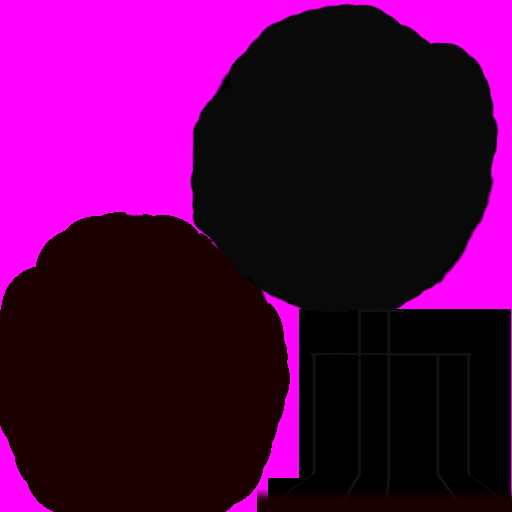
\includegraphics[width=0.6\textwidth]{pic/pan.png}
  \caption{Rendering sample of the pan.}
\end{figure}

\begin{figure}[h!]
  \centering
  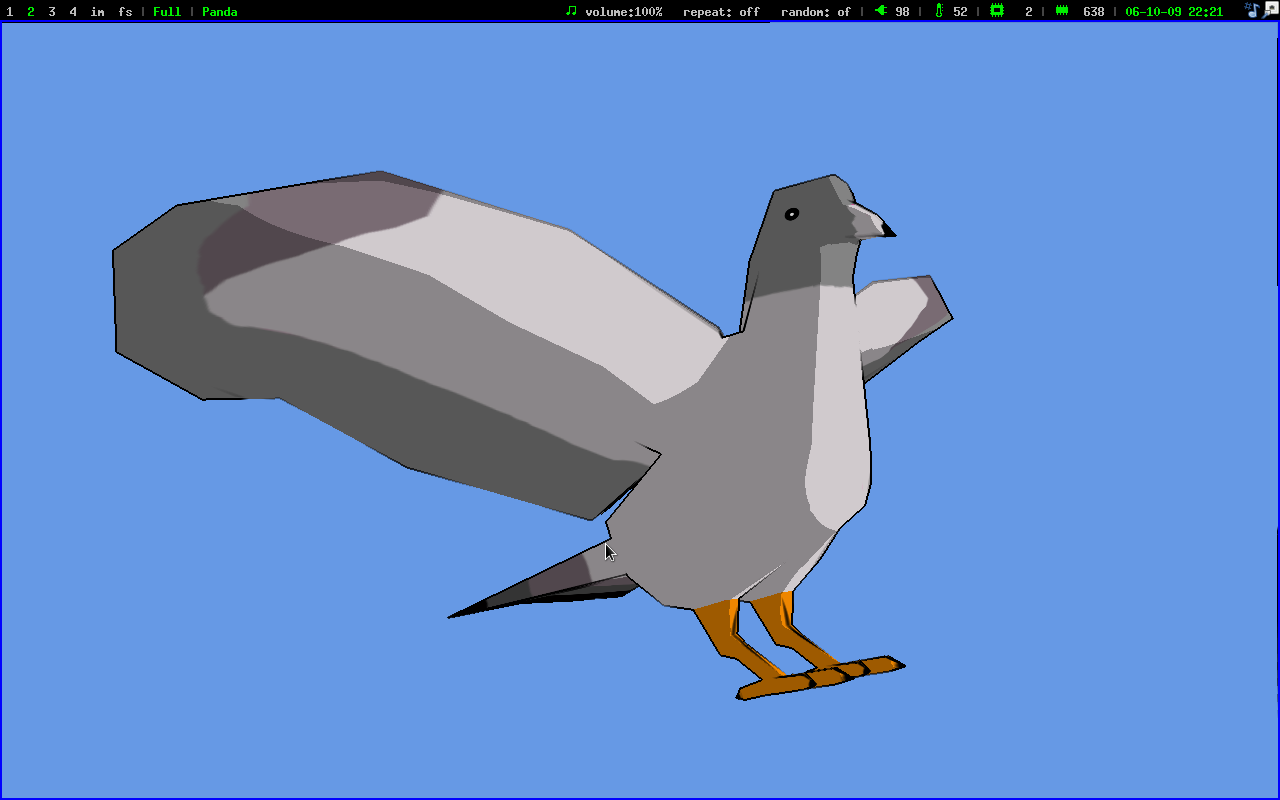
\includegraphics[width=0.6\textwidth]{pic/pigeon1.png}
  \caption{Sample of the pigeon rendered with our initial cartoon
    shaders enabled.}
\end{figure}

\begin{figure}[h!]
  \centering
  \includegraphics[width=0.6\textwidth]{pic/rolling_pin.png}
  \caption{Rendering sample of the rolling pin.}
\end{figure}

\begin{figure}[h!]
  \centering
  \includegraphics[width=0.4\textwidth]{pic/concept1.jpg}
  \caption{Concept art for the game.}
  \label{pic:sari}
\end{figure}


\begin{figure}[h!]
  \centering
  \includegraphics[width=0.9\textwidth]{pic/concept2.png}
  \caption{Concept art for the game.}
  \label{pic:jp}
\end{figure}

\section{Conclusion and future work}

During this project we developed a funny game that allows us to
experience the fun of the childs play of chasing pigeons in a wicked
way. The game provides an enjoyable game play while the player
discovers how the complex behaviour of the pigeons cause them to react
in different ways to his actions and learns how to use this to achieve
his goals.

From a personal point of view, developing this game was quite a lot of
effort, and, to be honest, exceeded the time-investment expected for
it. We wrote almost 12k lines of carefully crafted Python code but,
what was more educating, explored the frontiers of programming
languages, software design, game architecture. Also, we --sometimes
painfully-- learnt how it is hard to meet the deadlines in these kind
of project and how important the cooperation between programmers,
artists, and other roles in a game development team is for
the success of the final work.

Still, we feel that there is more work to do and it would a pity to
stop the project now. There are two ways in which the software could
be improved:
\begin{enumerate}
\item Firs of all, we would like to turn this kind of one-level (but
  still fun) demo into a real game that provides hours of joy. For
  this, we would like to get better graphics by fixing the texturing
  issues, adding the missing animations --like boy jumping, pigeon
  eating, etc.-- and, definitely, having few different scenarios. The
  later would allow for a more increasingly challenging game-play with
  inter-level bonuses, power-ups, etc. We also have some sounds in the
  data folder that we did not integrate in the game because of the
  lack of time.

  Also, the code was ready to add some nice features with trivial
  effort like local multi-player game-play --both cooperatively and
  competitive-- but the timing constraints of the project did not
  allow us to implement them. It would be nice to get them ready
  eventually. Other more complex features such as networked game-play
  would require a deeper time investment and engine work:

\item Second, we had a very nice time developing the game engine. We
  believe that there is a lot of potential in it but there is more
  effort needed, both in design and keyboard-punching. We have further
  ideas on how to improve it that we could not deeply describe in this
  brief document. We would like to keep exploring Python's magic to
  build the tools needed for non-expert programmers to correctly use
  the system without understanding the complex concepts on which it
  lies. Also, while we supported both slot-signal based and named
  centralized events we usually favoured the first. While good in many
  ways, sometimes it added complexity to the object mesh. We have some
  ideas on how to keep diminishing these drawbacks and also extend the
  usage of named events bounded to the hierarchical event manager.
  And also on how to add the proper tools to definitely
  integrate pain and boilerplatelessly the mixin based Entity
  system together with named events. Together with polishing the wrappers of
  the lower level libraries, it could be possible to come up with a
  very nice engine where the user could concentrate on describing the
  high level logic of his game in the form of entities and more
  abstracted states without ever caring about low level issues.

  Together with Python's impressive introspection features this leads
  us to imagine graphical point-and-click tools for game development
  built relatively easily on top of this system. Also, we would like
  to explore the possibilities to add auto-magical networking features
  under the entity system, so the games can go online with almost no
  effort. Further, it could be possible also to get rid of Python's
  performance bottleneck moving a lot of the code of the
  under-end-user-layers of the engine to more efficient compiled typed
  languages. And also eventually substitute the Panda3D and ODE
  dependencies for more preferred ones like Ogre3D and Bullet engine.

\end{enumerate}

As you can see there are many ideas --someones just too crazy-- to
continue the development of this game and its engine. Because we have
some other personal and professional projects and a personal life,
you can take this as an open request for collaboration to the to the
Game Development Club in UTU ;)

\bibliography{articulo}{}
\bibliographystyle{unsrt}


% \begin{thebibliography}{10}
% \bibitem{RFC1738}
% T.~Berners-Lee, L.~Masinter, and M.~McCahill,
% \newblock ``{U}niform {R}esource {L}ocators ({URL}),''
% \newblock RFC 1738, Internet Engineering Task Force, Dec. 1994,
% \newblock \url{http://ds.internic.net/rfc/rfc1738.txt}; accessed August 23,
%   1997.
% \end{thebibliography}

\end{document}
